Nesta seção explicamos as duas integrações que fizemos com exercícios-pro-\newline gramas que envolviam física, dados em disciplinas de introdução a computação na Poli. Os enunciados estão disponíveis no diretório deste projeto e também podem ser encontrados nas referências desta monografia.

\subsection{Configuração}

Para exemplificar uma possível utilização do Physimulation, fizemos duas integrações com EP's. A primeira foi com o Angry Bixos, dado no primeiro semestre deste ano, uma simulação de lançamento de objetos semelhante ao jogo \textit{Angry Birds}. A segunda integração foi com EP Apollo 13, dado no primeiro semestre de 2011. \\

Em ambos os exercícios, são lidos arquivos {\tt .txt} de entrada para que seja iniciada a simulação. Novamente em ambos os casos, a animação é exibida no próprio terminal. Na figura \ref{angry-bixos-oficial} há um exemplo válido de saída do EP Angry Bixos. \\

\begin{figure}[!htbp]
  \centering
	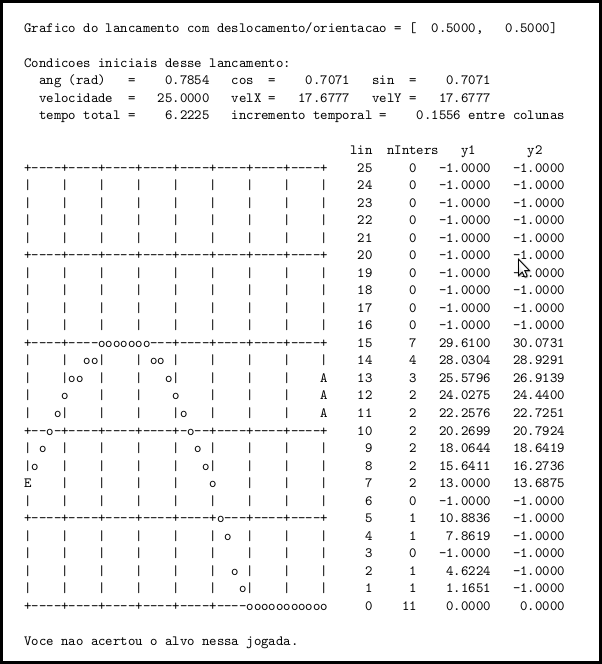
\includegraphics[scale=0.5]{images/angry-bixos-oficial-2.png}
	\caption{Exemplo de saída do EP Angry Bixos para Poli}
  \label{angry-bixos-oficial}
\end{figure}

Nas duas integrações, utilizamos o Physimulation para:

\begin{enumerate}
  \item Ler um arquivo no mesmo formato que o arquivo de entrada do EP;
  \item Gerar um arquivo {\tt config.rb} com as condições iniciais fornecidas no arquivo de entrada;
  \item Mostrar uma animação do resultado obtido.
\end{enumerate}

Por motivo de simulação, alguns dos valores de entrada foram ajustados para fazerem sentido no Physimulation.

\subsection{Angry Bixos}

O formato de arquivo de entrada a seguir foi extraído do próprio enunciado do EP Angry Bixos.

\begin{itemize}
  \item yE , vmax : 2 reais que definem a posição do estilingue e a velocidade máxima com que um bixo pode ser arremessado;
  \item yA , hA : 2 reais que definem a posição do alvo e sua altura;
  \item dist: real positivo que define a distância xA − xE entre o alvo e o estilingue.
  \item nBix: inteiro que define o número de bixos que podem ser lançados;
  \item nLin, nCol: 2 inteiros que definem as dimensões do gráfico a ser impresso (ambos devem ser múltiplos de 5);
  \item nUni: real utilizado como fator de escala das alturas (número de unidades de altura por linha);
  \item g: real negativo que define a aceleração da gravidade.
\end{itemize}

Após ler o arquivo de entrada, o Physimulation pede ao usuário que informe a intensidade do lançamento e o ângulo que o Bixo deverá ser lançado, assim como no EP. Esse processo é repetido até que acabe o número total de lançamentos, definido no arquivo de entrada. Caso o usuário acerte o alvo, a simulação é encerrada. Tanto no caso de sucesso quanto no caso de falha, são exibidas mensagens informando o usuário do resultado. Para executar a integração:

\begin{Verbatim}[fontsize=\footnotesize]
 $ cd <<DIR_PHYSIMULATION>>/Simulation/integracao-ep/angry-bixos
 $ ruby integracao-angry-bixos.rb 
\end{Verbatim}

\begin{figure}[H]
  \centering
	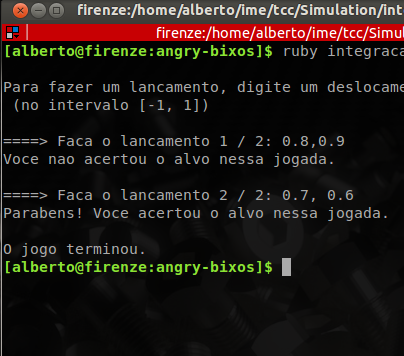
\includegraphics[scale=0.6]{images/angry-bixos-3.png}
	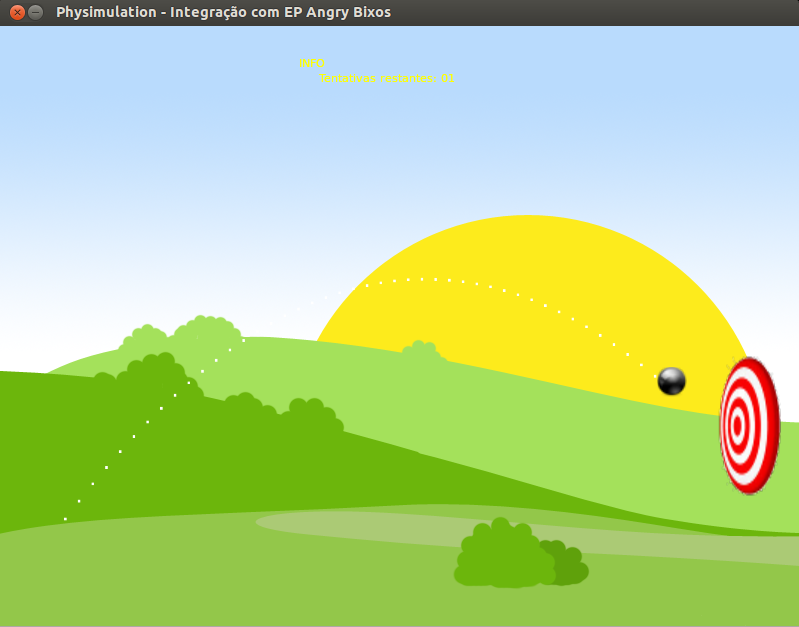
\includegraphics[scale=0.22]{images/angry-bixos-4.png}
	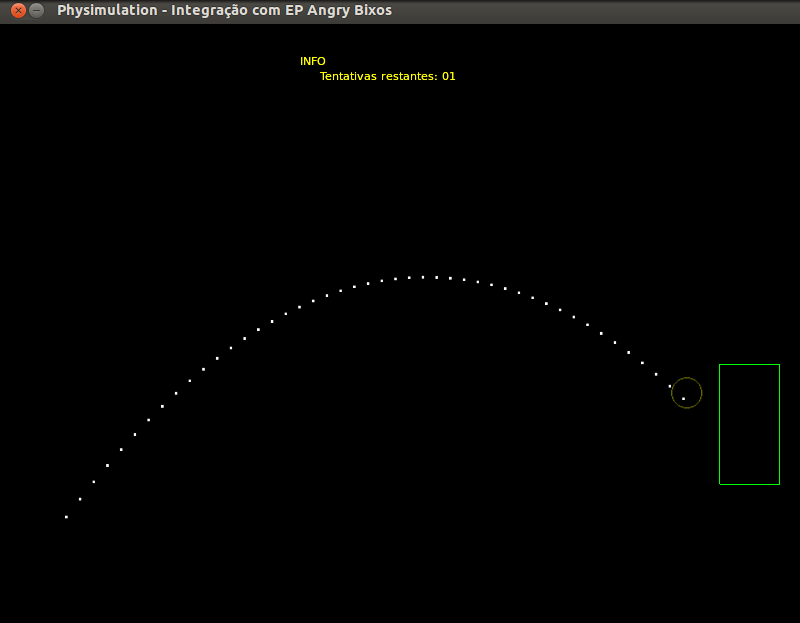
\includegraphics[scale=0.22]{images/angry-bixos-4E.png}
	\caption{Integração com EP Angry Bixos}
  \label{int-angry}
\end{figure}

\subsection{Apolo}

O formato de arquivo de entrada a seguir também foi extraído do próprio enunciado do EP Angry Bixos.

\begin{itemize}
  \item z1) posição inicial de uma nave em coordenadas cartesianas;                    
  \item z2) as componentes (V\_X,V\_Y) do vetor velocidade inicial da nave;
  \item z3) tempo máximo de simulação;               
  \item z4) o intervalo dT entre um instante e o instante seguinte da simulação.
\end{itemize}

No caso do EP Apollo 13, integramos apenas com uma parte do exercício, em que é solicitado ao aluno mostrar a animação do movimento gravitacional no terminal. \\

Por padrão, o Physimulation irá executar a animação do arquivo {\tt\small entrada.txt}, que corresponde á trajetória livre de retorno (efeito \textit{slingshot}). Para executar a simulação: 

\begin{Verbatim}[fontsize=\footnotesize]
 $ cd <<DIR_PHYSIMULATION>>/Simulation/integracao-ep/apolo
 $ ruby integracao-apolo.rb 
\end{Verbatim}

\begin{figure}[H]
    \centering
	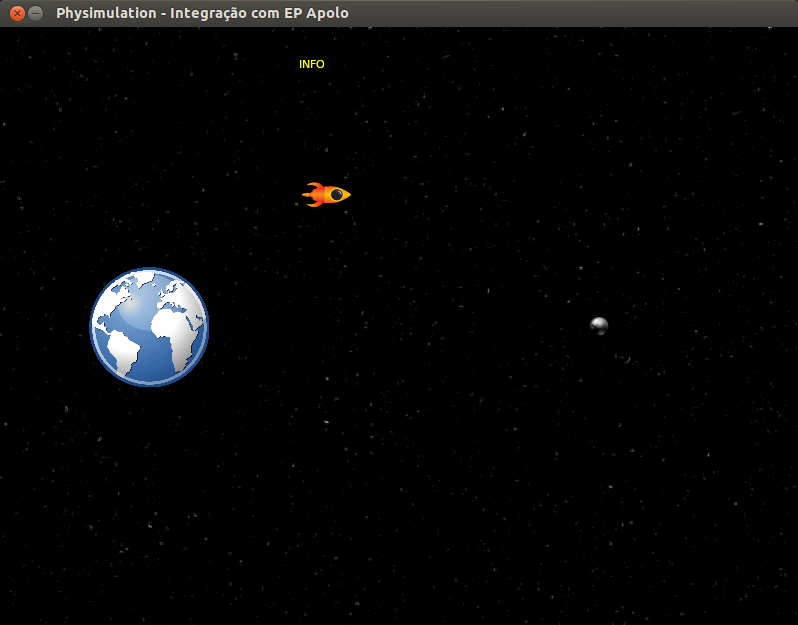
\includegraphics[scale=0.22]{images/apolo-4.png}
	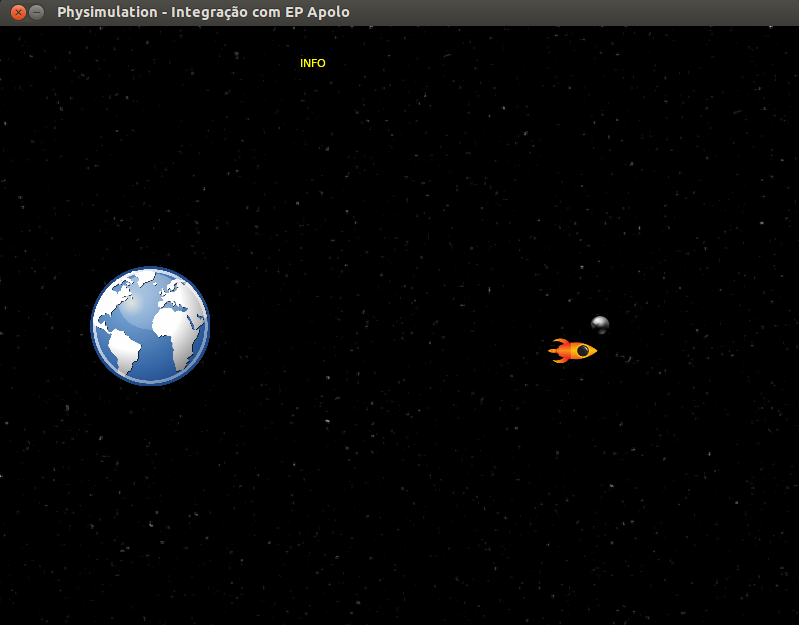
\includegraphics[scale=0.22]{images/apolo-6.png}
	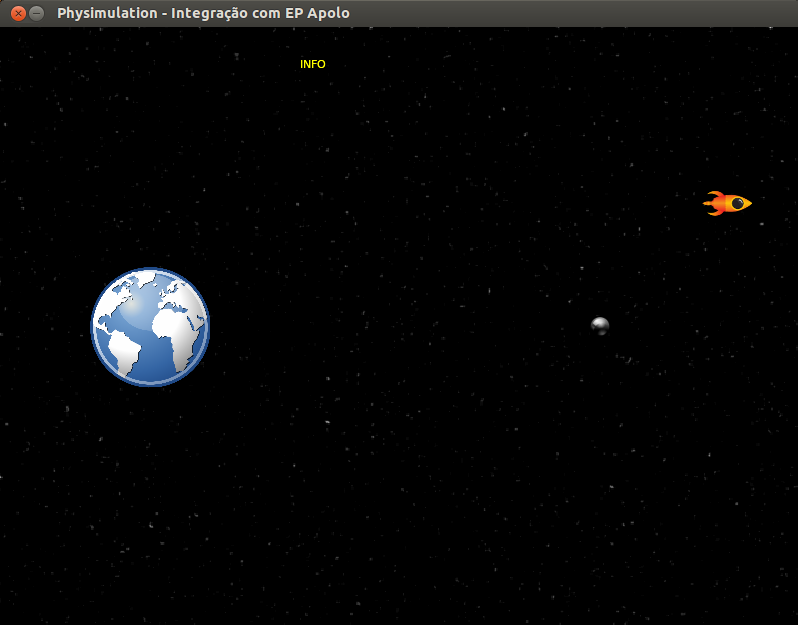
\includegraphics[scale=0.22]{images/apolo-3.png}
	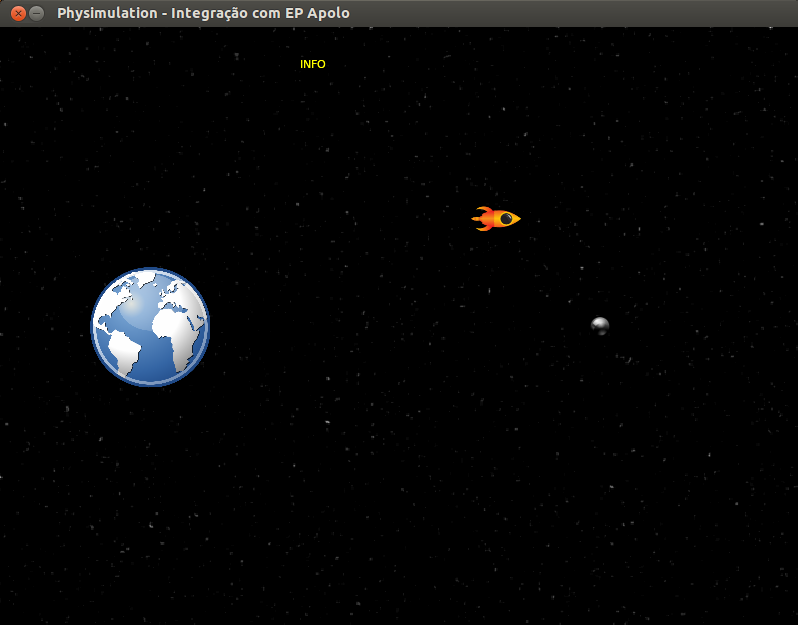
\includegraphics[scale=0.22]{images/apolo-2.png}
	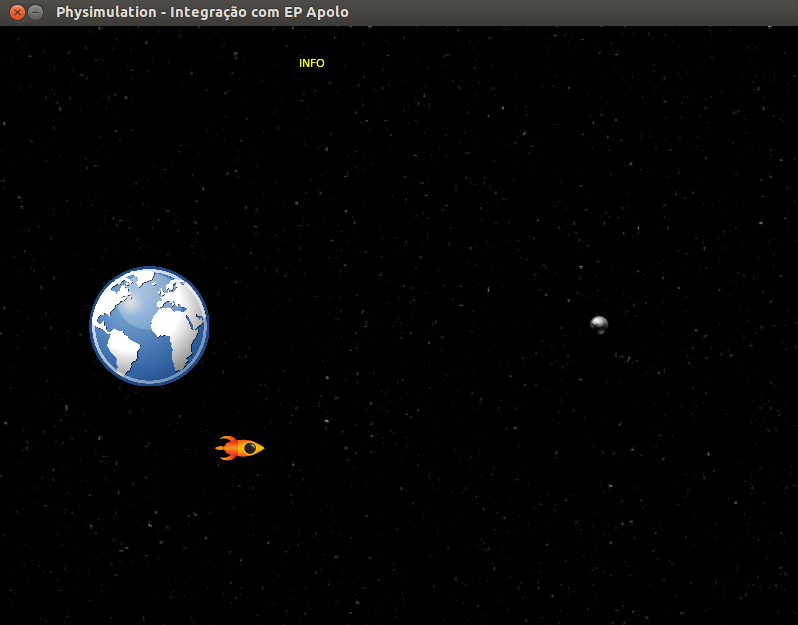
\includegraphics[scale=0.22]{images/apolo-1.png}
	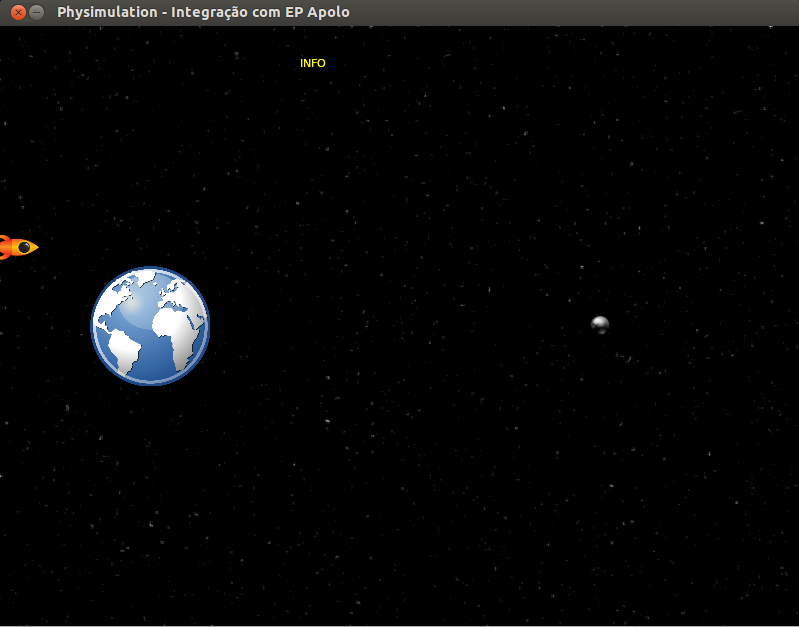
\includegraphics[scale=0.22]{images/apolo-5.png}
	\caption{Efeito \textit{slingshot} Integração com EP Apolo}
\end{figure}


